\section{Hardware: crucibles, nozzles, laser heads and kinematics}
\label{sec:hardware}

\subsection{Crucible-fed melt extrusion: the G3DP architecture}
\Cref{fig:g3dp} shows the generic architecture of a crucible-fed molten glass printer as embodied by G3DP (2015), G3DP2 (2017--2018) and G3DP3 (2023--present). Three independently controlled thermal zones are stacked vertically and decoupled mechanically from the motion system.

\begin{figure}[htbp]
  \centering
  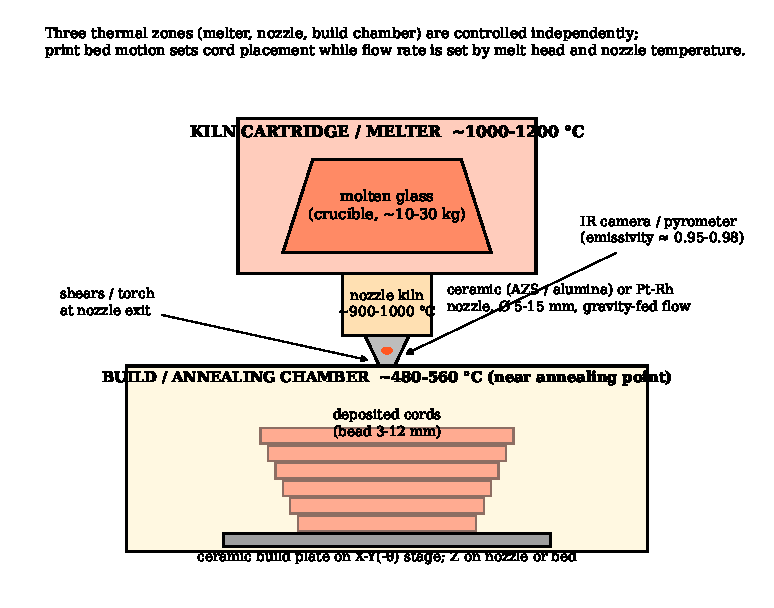
\includegraphics[width=0.9\linewidth]{fig_g3dp_schematic.pdf}
  \caption{Schematic of a crucible-fed molten-glass extrusion printer of the G3DP type. A refractory crucible in an electric kiln (melter, \SIrange{1040}{1200}{\celsius}) drains under its own head through a separately heated ceramic nozzle (\SIrange{800}{1010}{\celsius}) into an electrically heated build chamber held near the annealing point (\SIrange{480}{525}{\celsius}); the build plate moves in X--Y(--\(\theta\)) and Z. Flow is initiated and terminated by a concentric gas torch and compressed-air ring at the nozzle tip; an infrared camera views the cord through a ceramic-glass window. Dimensions and temperatures from \citet{klein2015,inamura2018,mit2024masonry,patent_us9919510}.}
  \label{fig:g3dp}
\end{figure}

\paragraph{Melter.} G3DP used an \SI{1800}{W} alumina--silica fibreboard kiln with FeCrAl wire heating a refractory crucible of \SI{2.1}{kg} capacity at \SIrange{1040}{1165}{\celsius}; the charge was either melted from nuggets over four hours and fined for two hours, or ladled in molten from a furnace \citep{klein2015}. G3DP2 replaced this with a \SI{6.5}{kW} kiln and a custom cast-alumina crucible of \SI{25.5}{kg} capacity operating at \SI{1090}{\celsius}, raising the reservoir-to-print-volume ratio from \SI{4.6}{\percent} to \SI{29}{\percent} and eliminating in-print refilling \citep{inamura2018}. The MIT patent describes idle and print set points of \SI{1750}{\degree}F and \SI{1850}{\degree}F (\SI{954}{\celsius} and \SI{1010}{\celsius}) for the melter, with silicon-carbide resistive heaters and type-S thermocouples \citep{patent_us9919510}. G3DP3 raised the maximum extrusion temperature to \SI{1200}{\celsius} and lowered the cost of the crucible and refractories \citep{mit2024masonry}; the feedstock kiln for recycled container glass is a separate double-walled crucible kiln conditioned at \SIrange{1190}{1218}{\celsius} for twelve hours before gathering \citep{stern2024cgc}.

\paragraph{Nozzle.} The nozzle is the interface between the thermal and kinematic systems and the component that limits campaign length. G3DP machined its nozzle from bulk alumina bisque, sealed to the crucible with refractory mortar, and heated it with a \SI{300}{W} nozzle kiln to \SI{1010}{\celsius} (\SI{800}{\celsius} to hold flow) \citep{klein2015}. G3DP2 used a solid-alumina nozzle of \SI{11.5}{mm} bore, lengthened for insulation and widened to keep resistance down, heated by resistive wire on a silicon-carbide mandrel in a structural refractory housing at \SI{800}{\celsius} idle and \SI{915}{\celsius} to start flow; a concentric gas manifold at the tip either burns propane to initiate flow or blows compressed air to freeze it, and the tip cone angle was increased from \SIrange{30}{45}{\degree} to reduce asymmetric wetting \citep{inamura2018}. Even so, nozzle joinery dictated print campaigns of two to three weeks \citep{inamura2018}. The press coverage of G3DP describes the nozzle material as alumina--zirconia--silica (AZS) \citep{oxman_platform}, the fused-cast refractory whose corrosion mechanism (alkali diffusion into the glassy phase, exudation, pore formation) has been reviewed recently \citep{zircorr2025}. G3DP3 redesigned the nozzle for higher temperature and for a \SI{13}{mm} nominal wall \citep{mit2024masonry,stern2024cgc}. Evenline's public machine description is a ceramic nozzle printing at \SI{2000}{\degree}F (\SI{1093}{\celsius}) \citep{evenline_web}.

\paragraph{Build chamber.} G3DP printed into a \SI{3300}{W} kiln derived from a Skutt GlazeTech, with a Neoceram ceramic-glass window and fibreboard skirts sealing the moving carriage \citep{klein2015}. G3DP2's chamber is a \SI{12}{kW} kiln of \qtyproduct{1100 x 1100 x 500}{mm} interior held at \SI{480}{\celsius}, with double-pane Neoceram doors and a \qtyproduct{400 x 400}{mm} floor opening through which the print-bed support tube passes; a \SI{13}{mm} Duraboard shield on the Z-actuator seals the opening while the bed translates and rotates \citep{inamura2018}. Total power of the G3DP2 thermal module is \SI{19}{kW} peak and \SI{15}{kW} during printing \citep{inamura2018}. After printing the object is soaked at \SI{525}{\celsius} for about five minutes and transferred to an external annealing oven so that the printer can be reused \citep{inamura2018}.

\paragraph{Kinematics.} G3DP moved the entire kiln cartridge on a steel carriage in X--Y with stepper motors (\SI{280}{\newton\centi\metre} holding torque) and moved the bed in Z, controlled by an Arduino/RAMPS stack and Repetier firmware \citep{klein2015}. G3DP2 inverted the architecture: the thermal module is stationary and the bed moves on a four-axis CNC (THK KR-46 linear actuators, a Bell-Everman rotary stage, Teknic ClearPath closed-loop servos, TinyG controller) designed to a positional tolerance of \(\pm\)\SI{1.0}{mm}, i.e.\ \SI{10}{\percent} of the \SI{10}{mm} filament \citep{inamura2018}. The rotary A-axis keeps the deposition direction constant relative to the stationary nozzle so that the viscous cord is not sheared by a change of pull direction---the core claim of the MIT patents \citep{patent_us9919510,patent_us10464305}. Measured repeatability across ten \SI{200}{mm} cylinders was a diameter range of \SI{0.7}{mm} (\SI{0.3}{\percent}) with a mean shrinkage of \SI{1.4}{\percent} \citep{inamura2018}. Jerk-limited acceleration on the rotary axis caused wall thickening at inflection points, so production parts were printed with three axes \citep{inamura2018}. G3DP3's proven envelope is \qtyproduct{325 x 325 x 380}{mm}, bead height \SIrange{3.0}{6.0}{mm}, bead width \SIrange{9}{16}{mm}, feed rate \SIrange{6}{20}{mm/s}, minimum path radius \SIrange{6}{15}{mm}, maximum overhang \SIrange{30}{35}{\degree} \citep{mit2024masonry}.

\subsection{Cane-fed hot-nozzle extrusion}
The cane-fed architecture inverts the thermal-mass problem: instead of holding tens of kilograms molten, it melts only the tip of a solid rod. Maple Glass Printing's Maple~2 and Maple~3 (2022--2023) feed one-metre soda-lime canes mechanically into a stationary nozzle at \SIrange{900}{1000}{\celsius} and deposit onto a moving build plate; the \SI{1.5}{mm} nozzle lays down beads up to \SI{2.0}{mm} high with layer resolution down to \SI{0.1}{mm}, in a \qtyproduct{170 x 200 x 300}{mm} volume, and the whole machine draws less power than a hair dryer because only a few millimetres of glass are hot at any moment \citep{maple_ammedia,maple_aniwaa,threednatives2025}. The Maple~4 (2025) is a \qtyproduct{736 x 600 x 985}{mm}, \SI{100}{kg} desktop unit with a \qtyproduct{200 x 200 x 300}{mm} volume, mesh bed levelling, a magnetic bed and a nozzle approaching \SI{1000}{\celsius} \citep{threednatives2025,maple_web}. The company also built a ``Vitri-Glass'' cane-drawing machine that melts recycled cullet in a crucible and pulls cane to specification, closing the material loop, with the caveat that coloured cullet must be segregated \citep{maple_ammedia}. Micron3DP's earlier machines (2015--2021) used an all-metal high-temperature extruder with \SI{100}{\micro\metre} layers, a \qtyproduct{200 x 200 x 300}{mm} volume, and claimed soda-lime at \SI{850}{\celsius} and borosilicate at \SI{1640}{\celsius} \citep{micron3dp_acers,micron3dp_3dprint2017}; the technical details were withheld pending patents and the company's alpha units of 2017--2021 were not followed by a public product. Corning's 2016 application describes the industrial form of the concept: a barrel-and-nozzle crucible of 80/20 platinum--rhodium heated by induction, fed with rigid rods of \SI{1}{mm} to over \SI{125}{mm} diameter, extruding controlled beads onto a platform; it was abandoned without grant \citep{patent_corning2021}. Because the cord in a cane-fed machine is thin (\SIrange{0.5}{2}{mm}) it freezes within seconds in air (\cref{fig:cooling}); this permits bridges and overhangs but produces stressed parts that require a post-anneal, and it limits optical clarity because the many fine layer seams scatter light---an effect already noted in comparing the Micron3DP and G3DP outputs \citep{inamura2018}.

\subsection{Laser filament, fibre and rod deposition heads}
\Cref{fig:laserhead} shows the generic laser filament head. The CO$_2$ laser at \SI{10.6}{\micro\metre} is absorbed within a few micrometres of the glass surface, so the melt zone is heated from the outside and the process is limited by conduction through the low-conductivity filament.

\begin{figure}[htbp]
  \centering
  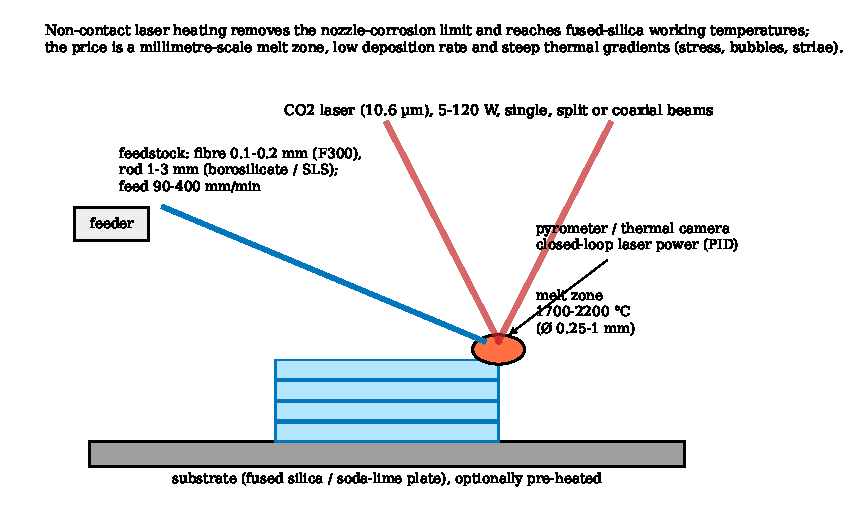
\includegraphics[width=0.85\linewidth]{fig_laser_filament_schematic.pdf}
  \caption{Schematic of a laser filament-fed glass deposition head (digital glass forming, laser glass deposition, direct glass laser deposition). A fibre or rod is fed at \SIrange{90}{400}{mm/min} into the focus of one or more CO$_2$ beams (\SIrange{5}{120}{W}); the melt zone of \SIrange{0.25}{1}{mm} diameter at \SIrange{1700}{2200}{\celsius} wets the substrate or previous layer. Melt-pool temperature is measured by pyrometry or thermal imaging and fed back to laser power. Parameters from \citet{luo2017sodalime,witzendorff2018,kth2022bonding,lgd2024homog,lgd2025tempctrl,dgf2026control}.}
  \label{fig:laserhead}
\end{figure}

\paragraph{Missouri S\&T / Notre Dame (digital glass forming).} The original 2014 system fed \SI{1}{mm} rods by hand into a CO$_2$ beam; automated feeding followed with soda-lime filaments \citep{luo2014jmse,luo2017sodalime}, then fused quartz filaments with spectroscopic and pyrometric measurement of the melt \citep{luo2018quartz,luo2016spie}, and stripped SMF-28 telecommunication fibre of \SI{125}{\micro\metre} as a kilometre-long, inexpensive, bubble-free feedstock \citep{hostetler2018fiber,hostetler2018sff}. The workpiece sits on a heated build platform on a four-axis stage; laser power, feed rate and scan speed are the three governing parameters, and the temperature window between incomplete fusion (index inhomogeneity) and reboil (bubbles) is narrow \citep{luo2017sodalime}. Side injection of the beam at the filament--substrate interface raised deposition rate \citep{capps2021interface}, hollow tubes were printed \citep{dgf2023tubes}, and the 2026 controller work replaced the pyrometer with a thermal camera on an RT-Linux platform and demonstrated that constant laser power fails on multilayer walls whereas closed-loop power succeeds \citep{dgf2026control}. The Notre Dame group also uses CO lasers and couples the process with ultrafast-laser machining in a hybrid cell \citep{notredame_dgf,kinzel2025dgf}.

\paragraph{Laser Zentrum Hannover (laser glass deposition).} The LGD process melts quartz-glass fibre with a combined laser head; at \SI{120}{W} a continuous regime was found up to feed and axis speeds of \SI{300}{mm/min}, above which the fibre outran the melt, and crack-free cylinders were built \citep{witzendorff2018}. A coaxial head with the fibre fed through the centre of a ring-shaped beam was introduced to make the process direction-independent and to reduce residual stress, supported by a thermal simulation of the fibre \citep{lgd2021coaxial}. A 3-axis linear system with integrated rotary axis, lateral fibre feed at a defined angle, an on-axis camera and a beam camera for transmitted-wavefront inspection form the current platform; fully dense fused-silica specimens without pores or boundary layers and with \(R_a = \SI{21}{nm}\) at \SI{90}{mm/min} feed (\SI{20}{}--\SI{40}{nm} up to \SI{126}{mm/min}; \SI{220}{nm} and waviness at \SI{180}{mm/min}; unmeasurable waviness at \SI{396}{mm/min}) were produced, with a contour flank angle of \SI{14}{\degree} as the price of the smoothest surface \citep{lgd2024homog,lgd2022fibers,grotesk2022}.

\paragraph{KTH / Nobula (direct glass laser deposition).} The KTH system uses four focused beams from a \SI{25}{W} CO$_2$ laser (\SIrange{2.2}{5.3}{W} delivered, stable to \SI{+-2}{\percent}) in a coaxial arrangement giving a \SIrange{250}{400}{\micro\metre} hot zone; \SI{196 +- 2}{\micro\metre} Heraeus F300 fibre drawn on a fibre tower is fed at \SI{150}{\percent} of the geometric rate at print speeds of \SIrange{10}{100}{mm/min} with \SI{200}{\micro\metre} layers onto a \qtyproduct{25 x 25}{mm} fused-quartz plate; a \qtyproduct{10.5 x 3.5 x 21}{mm}, 105-layer wall showed no stress birefringence and a material loss of \SI{-1.6 +- 2}{\percent} \citep{kth2022bonding}. The same head printed 5\(\times\)5 fused-silica microlens arrays in under ten seconds per lens with \(R_a = \SI{0.12}{nm}\) and uniform focal lengths \citep{kth2024microlens}. Nobula's commercial printer is specified at up to \SI{2200}{\celsius}, \qtyproduct{180 x 180 x 100}{mm}, \SI{0.1}{mm} Z resolution, \SIrange{100}{250}{\micro\metre} feature resolution and a \qtyproduct{1000 x 400 x 600}{mm}, \SI{50}{kg} footprint \citep{nobula_aniwaa,nobula_fabbaloo,threednatives2025}.

\paragraph{TU Ilmenau and TU Darmstadt (rod-fed).} Fr{\"o}hlich, Hildebrand and Bergmann used a CO$_2$ laser to create a melt pool on the substrate and fed borosilicate and soda-lime rods into it to build 3D structures \citep{froehlich2022}, and Seel et al.\ (TU Darmstadt) demonstrated ``fused glass deposition modelling'' of soda-lime rod onto float-glass plates for all-glass building connections \citep{seel2018}; a 2024 study designed printed glass point fixings on this basis \citep{pointfixings2024}. Both are relevant to the printing-on-sheet application that Evenline later demonstrated with a crucible-fed machine \citep{stern2024cgc}.

\paragraph{Coaxial wire and powder DED (IOE-CAS Chengdu, SCUT).} The Chinese Academy of Sciences group built a coaxial powder-fed laser DED head for quartz glass and reached \SI{72.4 +- 6.0}{MPa} flexural strength, \SI{95}{\percent} of conventional quartz \citep{lang2024}, then added coaxial wire feeding with PID closed-loop control of laser power from melt-pool temperature, which produced denser surfaces than constant powers of \SI{120}{W} or \SI{140}{W} \citep{lgd2025tempctrl}. The Clemson/SCUT route prints a water-based silica paste and melts it in situ with a CO$_2$ laser, avoiding a furnace step \citep{ieee2019dlm,paste2024}.

\subsection{Powder-bed and blown-powder laser melting hardware}
Nottingham's Centre for Additive Manufacturing processed soda-lime powder (\(\Tg = \SI{575}{\celsius}\), liquidus \SI{1280}{\celsius}) in a commercial fibre-laser L-PBF system with the substrate held at \SI{250}{\celsius} to limit thermal cracking; the process window was defined in terms of volumetric energy density \(E = P/(v\,h\,t)\), parts had \SI{12.1}{\percent} average porosity and a \SI{6.5}{MPa} mean flexural strength, and a \SI{650}{\celsius}, five-hour heat treatment improved translucency \citep{datsiou2019,datsiou2021}. Irregular (milled) soda-lime powder reached \SI{95}{\percent} relative density at Fudan \citep{slmirregular2023}; alkali-borosilicate powder was processed by Zeiss and TU Ilmenau over the whole window from open-pored (\SI{38}{\percent}) to vitrified (\SI{94}{\percent}) density, with characteristic ``vitrification strands'' from the line-wise energy input \citep{boro2025laser}; and Fateri and Gebhardt's 2014--2015 work reached \SI{93}{\percent} \citep{fateri2015}. Crack-free single beads and monolayers of silica glass on a silica substrate were shown by Khmyrov et al.\ \citep{khmyrov2016}. Blown-powder DED of soda-lime onto soda-lime bottles, with an adhesive tape layer to hold the powder on the transparent substrate and a cracking threshold at \SI{115}{W}, is proposed for one-step packaging decoration \citep{spirrett2023}. A finite-difference densification model predicts monolayer consolidation within \SI{2}{\percent} of experiment and shows that finer powder and higher preheat both help \citep{slmsim2024}.

\subsection{Comparison matrix of glass AM modalities}
\Cref{tab:modalities} summarises the quantitative envelope of each modality as reported in the corpus. The columns follow the specification of this review: temperature, build volume, deposition rate, optical clarity, surface roughness and strength.

\begin{sidewaystable}[p]
  \centering\scriptsize
  \caption{Comparison matrix of glass AM modalities. Direct (molten at deposition) modalities are listed first; indirect routes are included for contrast. ``n.r.'' = not reported in the corpus. Transmission values are qualitative where no spectrophotometric data were published.}
  \label{tab:modalities}
  \begin{tabular}{@{}L{2.6cm}L{2.3cm}L{2.4cm}L{2.5cm}L{2.6cm}L{2.5cm}L{3.0cm}L{2.2cm}@{}}
    \toprule
    Modality (systems) & Glass / process temperature & Build volume & Deposition rate & Optical clarity & Surface roughness \(R_a\) & Strength & Key refs.\\
    \midrule
    Crucible-fed melt extrusion (G3DP, G3DP2, G3DP3/Evenline) & Soda-lime; melter \SIrange{1040}{1200}{\celsius}, nozzle \SIrange{915}{1010}{\celsius}, chamber \SIrange{480}{525}{\celsius} & \qtyproduct{250 x 250 x 300}{mm} (G3DP); \qtyproduct{320 x 320 x 350}{mm} (G3DP2); \qtyproduct{325 x 325 x 380}{mm} (G3DP3) & \SI{240}{}--\SI{570}{mm^3/s}; \SI{2.2}{}--\SI{5.2}{kg/h}; feed \SIrange{6}{20}{mm/s} & Transparent; fully dense; \SI{10}{mm} cords give lens-like refraction and caustics; polished faces clear & Layer corrugation of bead scale (\SIrange{3}{6}{mm}); as-printed \(R_a\) n.r.; cut faces polished with CeO\(_2\) & Flexural \SIrange{41}{56}{MPa} annealed, \(E = \SIrange{65}{74}{GPa}\); \SI{40}{\percent} anisotropy; masonry: initial fracture \SIrange{3.6}{42.3}{MPa}, ultimate \SIrange{64}{118}{MPa} & \citep{klein2015,inamura2018,mit2024masonry,stern2024cgc}\\
    Cane-fed hot-nozzle extrusion (Maple 2/3/4; Micron3DP) & Soda-lime (recycled cane); nozzle \SIrange{900}{1000}{\celsius}; Micron3DP claims \SI{850}{\celsius} soft and \SI{1640}{\celsius} borosilicate & \qtyproduct{170 x 200 x 300}{mm} (Maple 3); \qtyproduct{200 x 200 x 300}{mm} (Maple 4, Micron3DP) & Small parts in under \SI{1}{h}; bead \SI{1.5}{mm}, layer \SIrange{0.1}{2.0}{mm}; Micron3DP est.\ \SI{0.05}{kg/h} & Translucent to transparent; fine seams scatter & n.r.; layer texture \SIrange{0.1}{2}{mm} & n.r. & \citep{maple_ammedia,maple_aniwaa,threednatives2025,micron3dp_acers,inamura2018}\\
    Laser filament / fibre deposition (DGF, LGD, DGLD/Nobula) & Fused silica \SIrange{1900}{2200}{\celsius}; soda-lime and borosilicate on heated plate; CO\(_2\) \SIrange{2}{120}{W} & Lab: \qtyproduct{25 x 25}{mm} plates, walls to \SI{21}{mm}; Nobula \qtyproduct{180 x 180 x 100}{mm} & Feed \SIrange{90}{400}{mm/min} of \SIrange{0.1}{1}{mm} filament (\(\sim\)\SI{0.5}{}--\SI{15}{mm^3/min}) & Transparent, fully dense; index homogeneity measured; no birefringence (KTH) & \SI{21}{nm} at \SI{90}{mm/min}, \SIrange{20}{40}{nm} to \SI{126}{mm/min}, \SI{220}{nm} at \SI{180}{mm/min} (LGD); \SI{0.12}{nm} microlenses (KTH) & Quartz coaxial DED \SI{72.4 +- 6.0}{MPa} (\SI{95}{\percent} of bulk) & \citep{luo2017sodalime,luo2018quartz,witzendorff2018,lgd2024homog,kth2022bonding,kth2024microlens,lang2024,nobula_aniwaa}\\
    Laser powder-bed fusion (Nottingham, Fudan, Zeiss/Ilmenau, FH Aachen) & Soda-lime, borosilicate, silica powder; substrate \SI{250}{\celsius}; \SI{100}{W}, \SI{37}{mm/s} & Commercial L-PBF platforms (\(\sim\)\SI{100}{mm} scale) & Track-wise; hatch scanning; bulk rates n.r. & Opaque (porosity, partly fused particles); translucent after \SI{650}{\celsius} heat treatment & Powder-scale roughness; n.r. & Flexural \SIrange{6.2}{6.9}{MPa}; porosity \SI{12}{\percent}; density \SIrange{93}{95}{\percent} & \citep{datsiou2019,datsiou2021,slmirregular2023,boro2025laser,fateri2015}\\
    Powder-fed / wire-fed DED, paste + in-situ laser (Nottingham, IOE-CAS, SCUT) & Soda-lime on bottles; quartz powder/wire; \SIrange{115}{140}{W}; \SIrange{500}{700}{mm/min} & Bottle surfaces; small blocks & Single tracks; multi-pass layers & Semi-transparent tracks; transparent fused silica (paste + laser) & n.r. & Quartz \SI{72.4}{MPa} (coaxial powder) & \citep{spirrett2023,lang2024,lgd2025tempctrl,paste2024,ieee2019dlm}\\
    \midrule
    Indirect: vat photopolymerisation of silica nanocomposite + sinter (Kotz, Glassomer); micro-CAL & Print \SI{25}{\celsius}; debind + sinter \SI{1300}{\celsius}, \SI{50}{h} & Desktop SLA volumes; parts cm-scale after \(\sim\)\SI{15}{\percent} linear shrinkage & \(\sim\)\SI{0.02}{kg/h} (est.) & Transparent fused silica & Few nm (CAL: \SI{6}{nm}) & Bulk fused silica; \SI{50}{\micro\metre} features (CAL) & \citep{kotz2017,toombs2022,inamura2018}\\
    Indirect: direct ink writing of silica sols (LLNL); thermoplastic FDM/FFD (Freiburg) & Print \SI{25}{\celsius}; sinter below silica melting; MIT-LL route \(\le\)\SI{250}{\celsius} & cm-scale & n.r. & Optical-grade; index homogeneity within commercial standards; GRIN possible & Polished to optical finish & Bulk fused silica; high-aspect-ratio (\(>\)480) vessels, \SI{250}{\micro\metre} walls & \citep{nguyen2017,destino2018,mader2021,acers2024recent}\\
    \bottomrule
  \end{tabular}
\end{sidewaystable}

Several conclusions are immediate from the table. Only the crucible-fed and laser-filament routes deliver transparent, fully dense glass directly, and they occupy opposite corners of the rate--resolution space: kilograms per hour at centimetre bead scale versus millilitres per hour at \SI{100}{\micro\metre} scale. Powder routes offer intermediate rates but sacrifice transparency and strength by an order of magnitude. The indirect routes match or exceed the laser-filament routes in resolution and surface finish but pay with a long furnace cycle, shrinkage and small part size. No process yet combines architectural scale with optical-grade surfaces; that gap is the central engineering opportunity identified in \cref{sec:outlook}.
